\documentclass[10pt,a4paper]{article}
\usepackage[utf8]{inputenc}
\usepackage[english]{babel}
\usepackage[activate={true,nocompatibility},final,tracking=true,kerning=true,spacing=true]{microtype}
\usepackage[plainpages=false,pdfpagelabels,unicode]{hyperref}
\usepackage{fullpage}
\usepackage{graphicx}
\usepackage{fancyhdr}
\usepackage{occi}


\setlength{\headheight}{13pt}
\pagestyle{fancy}

%  just a test
% default sans-serif
\renewcommand{\familydefault}{\sfdefault}

% no lines for headers and footers
\renewcommand{\headrulewidth}{0pt}
\renewcommand{\footrulewidth}{0pt}

% header
\fancyhf{}
\lhead{GFD-R}
\rhead{\today}

% footer
\lfoot{occi-wg@ogf.org}
\rfoot{\thepage}

% paragraphs need some space...
\setlength{\parindent}{0pt}
\setlength{\parskip}{1ex plus 0.5ex minus 0.2ex}

%\renewcommand\paragraph{%
%  \@startsection{paragraph}{4}{0mm}%
%     {-\baselineskip}%
%     {.5\baselineskip}%
%     {\normalfont\normalsize\bfseries}}

% some space between header and text...
\headsep 13pt

\setcounter{secnumdepth}{4}

\begin{document}

% header on first page is different
\thispagestyle{empty}

Draft \hfill  Gregory Katsaros, Intel\\
OCCI-WG \hfill  \\
\rightline {\today}\\

\vspace*{0.5in}

\begin{Large}
\textbf{Open Cloud Computing Interface -- Service Level Agreements}
\end{Large}

\vspace*{0.5in}

\underline{Status of this Document}

This document provides information to the community regarding the
specification of the Open Cloud Computing Interface. Distribution is
unlimited.


\underline{Copyright Notice}

Copyright \copyright ~Open Grid Forum (2009-2014). All Rights
Reserved.

\underline{Trademarks}

OCCI is a trademark of the Open Grid Forum.

\underline{Abstract}

This document, part of a document series, produced by the OCCI working
group within the Open Grid Forum (OGF), provides a high-level
definition of a Protocol and API. The document is based upon
previously gathered requirements and focuses on the scope of important
capabilities required to support modern service offerings.


This document, part of a document series, produced by the OCCI working group within the Open Grid Forum (OGF), provides a high-level definition of a Protocol and API in relation with the Service Level Agreements extension of the OCCI Core Model. The document is based upon previously gathered requirements and focuses on the scope of important capabilities required to support modern service offerings.

\newpage
\tableofcontents
\newpage

\section{Introduction}
%!TEX root = nml-base.tex

\section{Introduction}%
\label{sec:introduction}

This document describes the base schema of the Network Markup Language (NML).
Section~\ref{sub:classes} defines the NML classes and their attributes and parameters.
Section~\ref{sub:relations} describes the relations defined between NML classes.

An NML network description can be expressed in XML\cite{xml}, and RDF/XML\cite{rdfxml} syntax.
Section~\ref{s:xmlschema} describes the XSD schema for the XML syntax.
Section~\ref{s:owlschema} describes the OWL 2 schema for the RDF/XML syntax.

These basic classes defined in this document may be extended, or sub-classed, 
to represent technology specific classes.

Section~\ref{s:examples} provides example use cases. This section is informative. 
Only sections~\ref{s:schema}, \ref{s:identifiers}, \ref{s:syntax}, and appendices \ref{s:xmlschema} and \ref{s:owlschema} are normative and considered 
part of the recommendation.

Appendix~\ref{s:g800terms} is informative and explains the relation between terms defined in this document and those defined in the ITU-T G.800 recommendation~\cite{g800}.

\subsection{Context}
\label{sec:context}

The Network Markup Language (NML) has been defined in the context of research and 
education networks to describe so-called hybrid network topologies. The NML is defined
as an abstract and generic model, so it can be applied for other network topologies as well.
See \cite{gfd.165} for an detailed overview including prior work.

\subsection{Scope}
\label{sec:scope}

The Network Markup Language is designed to create a functional description of 
multi-layer networks and multi-domain networks. An example of a multi-layered 
network can be a virtualised network, but also using different technologies. 
The multi-domain network descriptions can include aggregated or abstracted network topologies.
NML can not only describe a primarily static network topology, but also its potential capabilities (services) 
and its configuration.

NML is aimed at logical connection-oriented network topologies, more precisely topologies
where switching is performed on a label associated with a flow, such as a VLAN, wavelength or time slot. 
NML can also be used to describe physical networks or packet-oriented networks, 
although the current base schema does not contain classes or properties 
to explicitly deal with signal degradation, or complex routing tables.

NML only attempts to describe the data plane of a computer network, not the control 
plane. It does contain extension mechanism to easily tie it with network provisioning 
standards and with network monitoring standards.

Finally, this document omits a definition for the terms \emph{Network} or \emph{capacity}. 
This has been a conscious choice. The term \emph{Network} has become 
so widely used for so many diverse meanings that it is impossible to create a 
definition that everyone can agree on, while still expressing something useful.
See \emph{Topology} for the concept of a network domain and a \emph{Link} with multiple 
sources and sinks for the concept of a local area network.
The term \emph{capacity} is used by different technologies in such a different 
way (e.g.\ including or excluding the header and footer overhead) that it is better 
to let technology-specific extensions make an explicit definition.

\subsection{Notational Conventions}%
\label{sec:rfc2119}

The keywords “\MUST{}”, “\MUSTNOT{}”, “\REQUIRED{}”, “\SHALL{}”, “\SHALLNOT{}”, 
“\SHOULD{}”, “\SHOULDNOT{}”, “\RECOMMENDED{}”, “\MAY{}”,  and “\OPTIONAL{}” are 
to be interpreted as described in \cite{rfc2119}.
% except that the words do not appear in uppercase. 

This schema defines classes, attributes, relations, parameters and logic.
Objects are instances of classes, and the type of an object is a class.

Names of classes are capitalised and written in italics (e.g.\ the \emph{Node} class).
Names of relations are written in camel case and in italics (e.g.\ the \emph{hasNode} relation).
Names of identifiers and string literals are written in monspaces font (e.g. \texttt{Port\_X:in}).

Diagrams in this document follow the diagrammatic conventions of UML class diagrams.
\begin{itemize}
\item A subclass-superclass relationship is represented by a line with hollow triangle shape pointing to the superclass.
\item A whole-part relationship is represented by a line with a hollow diamond shape pointing to the whole (group).
\item A entity-relationship is represented by a line, optionally with numbers at each end indicating the cardinality of the relation. A named entity-relationship has a verb next to the line, and a filled triangle pointing to the object of the verb. (e.g. the entitity-relationship
\nmlrelation{BidirectionalPort}{*}{hasPort}{2}{Port} is named \emph{hasPort}, and each \emph{BidirectionalPort} is related to exactly 2 \emph{Port}s, and each \emph{Port} may be associated with zero, one or more \emph{BidirectionalPort}s.)
\end{itemize}




\section{Notational Conventions}
All these parts and the information within are mandatory for
implementors (unless otherwise specified). The key words "MUST", "MUST
NOT", "REQUIRED", "SHALL", "SHALL NOT", "SHOULD", "SHOULD NOT",
"RECOMMENDED", "MAY", and "OPTIONAL" in this document are to be
interpreted as described in RFC 2119 \cite{rfc2119}.


% begin sla content

\section{Service Level Agreement}

The OCCI Service Level Agreements (OCCI SLAs) document describes how the OCCI Core Model \cite{occi:core} can be extended and used to implement a Service Level Agreement management API. This API allows for the creation and management of resources related with the realization of agreements between an OCCI-enabled cloud service provider and potential consumers of the provider’s resources. The introduced types and \hl{Mixin}s defined in this OCCI SLAs document are the following:


\begin{description}
\item[\hl{Agreement }] This resource represents the Service Level Agreement between the provider and the consumer. It includes the basic information for this contract and with the appropriate extensions (\hl{Mixin}s) it can be populated with further information. To this end, we introduce the \hl{AgreementTemplate} and the \hl{AgreementTerms Mixin}s which complement the SLAs with template tagging and terms specification respectively.

\item[\hl{AgreementLink }] This is a link entity that associates an \hl{Agreement} instance with any other \hl{Resource} instance.
\end{description}


\begin{figure}[!h]
	{\centering \resizebox*{0.8\columnwidth}{!}{{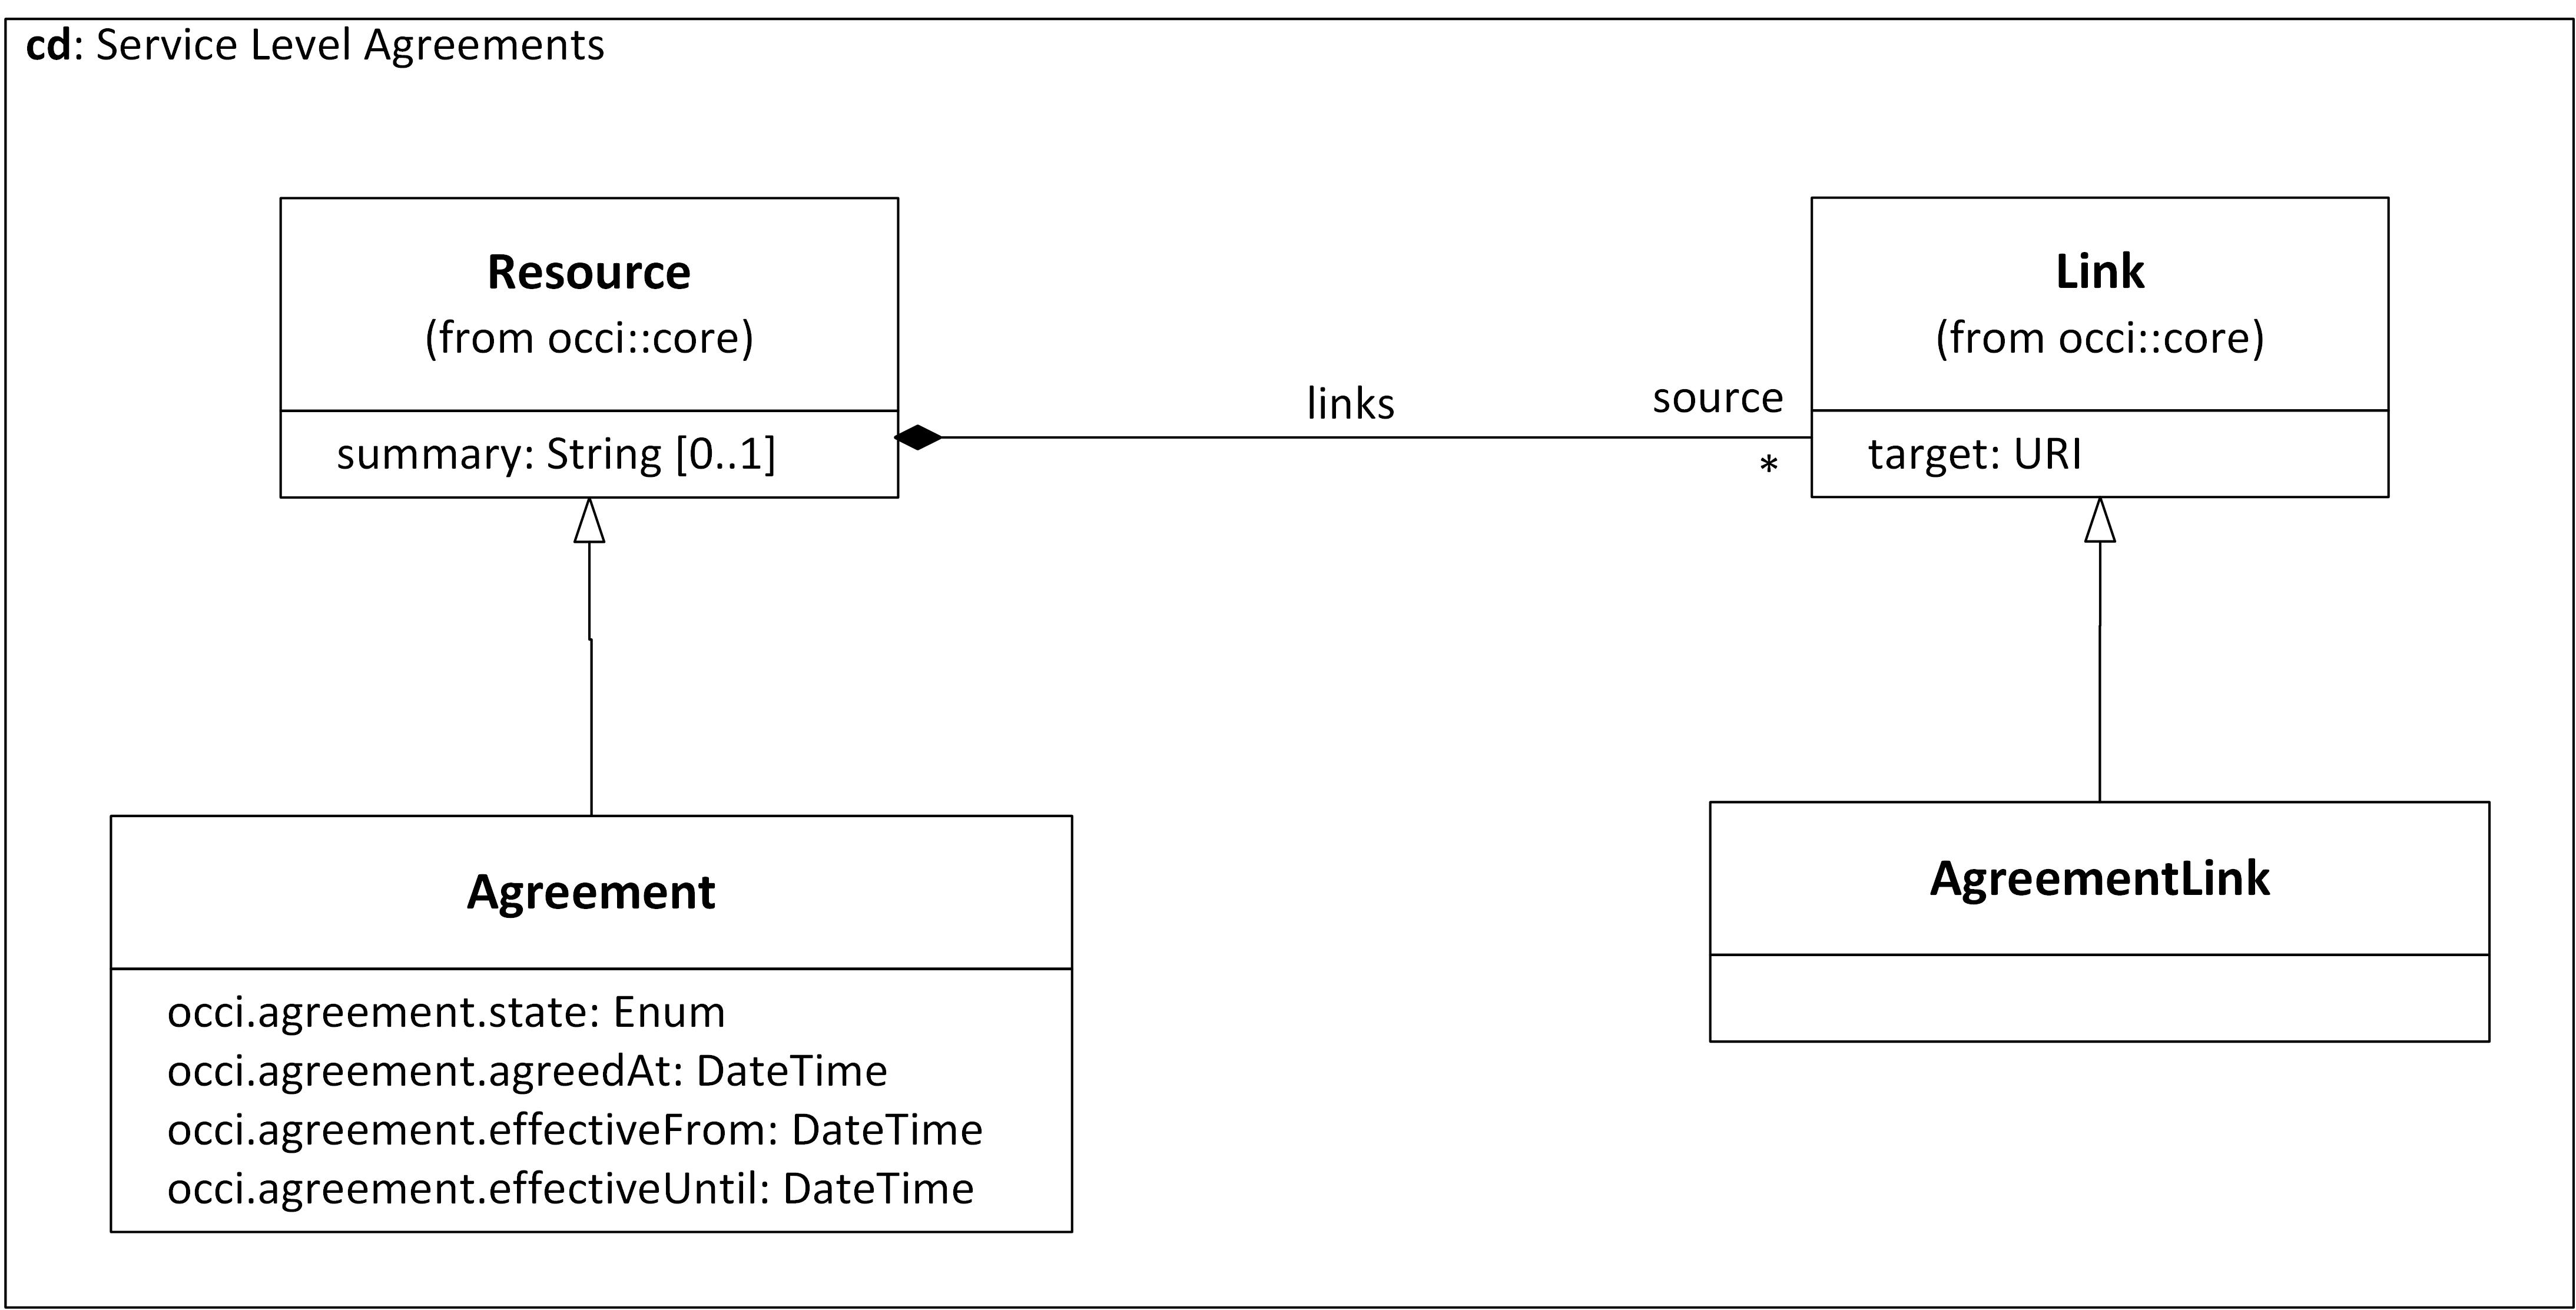
\includegraphics{figs/occi-slas-overview.jpg}}} \par}
	\caption{Overview diagram of OCCI Service Level Agreements types.}
	\label{fig:sla_uml}
\end{figure}

The \hl{Agreement} type is a sub-type of the OCCI Core Model's \hl{Resource}
base type and inherits all its attributes. The HTTP Protocol \cite{occi:http_protocol} and Text
Rendering \cite{occi:text_rendering} documents define how to serialize and interact with
these types using RESTful communication. Implementers are free to
choose what \hl{Resource} and \hl{Link} sub-types to implement. Those
that are supported by an implementation will be discoverable through
the OCCI Query Interface.

It is REQUIRED by the OCCI Core Model specification that every type instantiated which is a sub-type of a \hl{Resource} or a \hl{Link} (i.e., \hl{Agreement} and \hl{AgreementLink}) MUST be assigned a \hl{Kind} that identifies the instantiated type. To this end, each \hl{Kind} instance MUST be related to the \hl{Resource} or \hl{Link} base type’s \hl{Kind}. That assigned \hl{Kind} MUST be immutable to any client.

In the following table (Table~\ref{tbl:kinds-mixins}) the \hl{Kind} instances for the OCCI SLAs \hl{Resource}, \hl{Link} sub-types as well as the \hl{Mixin}s are introduced. For information on how to extend these types, please refer to the OCCI Core Model specification \cite{occi:core}. We also present related examples at the end of this document.


\mytablefloat{
	\label{tbl:kinds-mixins}The \hl{Kind} instances defined for
	the SLAs sub-types of \hl{Resource}, \hl{Link} and related \hl{Mixin}s.
	The base URL {\bf http://schemas.ogf.org/occi} has been replaced with
	{\bf $<$schema$>$} in this table for a better readability experience.
	}
	{
	\begin{tabular}{llll}
	\toprule
	Term & Scheme & Title & Related \hl{Kind} \\
	\colrule
	agreement &  $<$schema$>$/sla\# & A Service Level Agreement	& $<$schema$>$/core\#resource \\
	agreement\_link & $<$schema$>$/sla\# & \hl{Link} between a SLA and its associated resources	& $<$schema$>$/core\#link \\
	agreement\_tpl & $<$schema$>$/sla\# & \hl{Mixin} defining a SLA template collection	& - \\
	agreement\_term & $<$schema$>$/sla\# & \hl{Mixin} defining a Term collection for an agreement	& - \\
	\botrule
	\end{tabular}
}



The following sections describe the \hl{Agreement} and \hl{AgreementLink} types, with details about their attributes, states and actions. The \hl{AgreementTemplate} and \hl{AgreementTerm Mixin}s are also defined and presented. In the end, examples of OCCI SLAs instantiations are shown. These present several phases of the Service Level Agreement lifecycle, as well as specific instances of terms and service qualities.



\subsection{Agreement}

The \hl{Agreement} type represents a generic contract resource which holds the information related to a SLA between a cloud service consumer and a provider for the provisioned resources (e.g., compute, storage, network etc.). The \hl{Agreement} type inherits the \hl{Resource} base-type defined in the OCCI Core Model \cite{occi:core}. The \hl{Kind} instance assigned to the \hl{Agreement} type is \textit{http://schemas.ogf.org/occi/sla\#agreement}. An \hl{Agreement} instance MUST relate and expose this \hl{Kind}.

Table~\ref{tbl:agreement} describes the attributes defined by the \hl{Agreement} type through its \hl{Kind} instance. These attributes MUST be exposed by an instance of the \hl{Agreement} type. In Figure~\ref{fig:agreement-states} the allowed states of an \hl{Agreement} instance are presented. Those specific states MUST be assigned to an \hl{Agreement} instance by a cloud service provider SHOULD the implements the OCCI SLAs specification. The \hl{agreedAt}, \hl{effectiveFrom} and \hl{effectiveUntil} attributes MUST have an absolute datetime value (data, time or combined format) but MUST NOT represent a duration or time interval formated value.



\mytablefloat{
	\label{tbl:agreement}
	\hl{Attributes} defined for the \hl{Agreement} type.
}
{
	\begin{tabular}{lp{2.5cm}p{1cm}lp{6cm}}
	\toprule
	Attribute&Type&Multi\-plicity&Mutability&Description\\
	\colrule
	occi.agreement.state & Enum \{Pending, Accepted, Rejected, Suspended, Terminated\} & 1 & Immutable & Current state of the instance.\\
	occi.agreement.agreedAt & Datetime (ISO8601) & 0\ldots1 & Immutable & The point in time when the agreement was made. \\
	occi.agreement.effectiveFrom & Datetime (ISO8601) & 0\ldots1 & Mutable & The point in time when the agreement’s effectiveness begins. \\
	occi.agreement.effectiveUntil & Datetime (ISO8601) & 0\ldots1 & Mutable & The point in time when the agreement’s effectiveness ends. \\
	\botrule
	\end{tabular}
}


\begin{figure}[!h]
	{\centering \resizebox*{0.6\columnwidth}{!}{{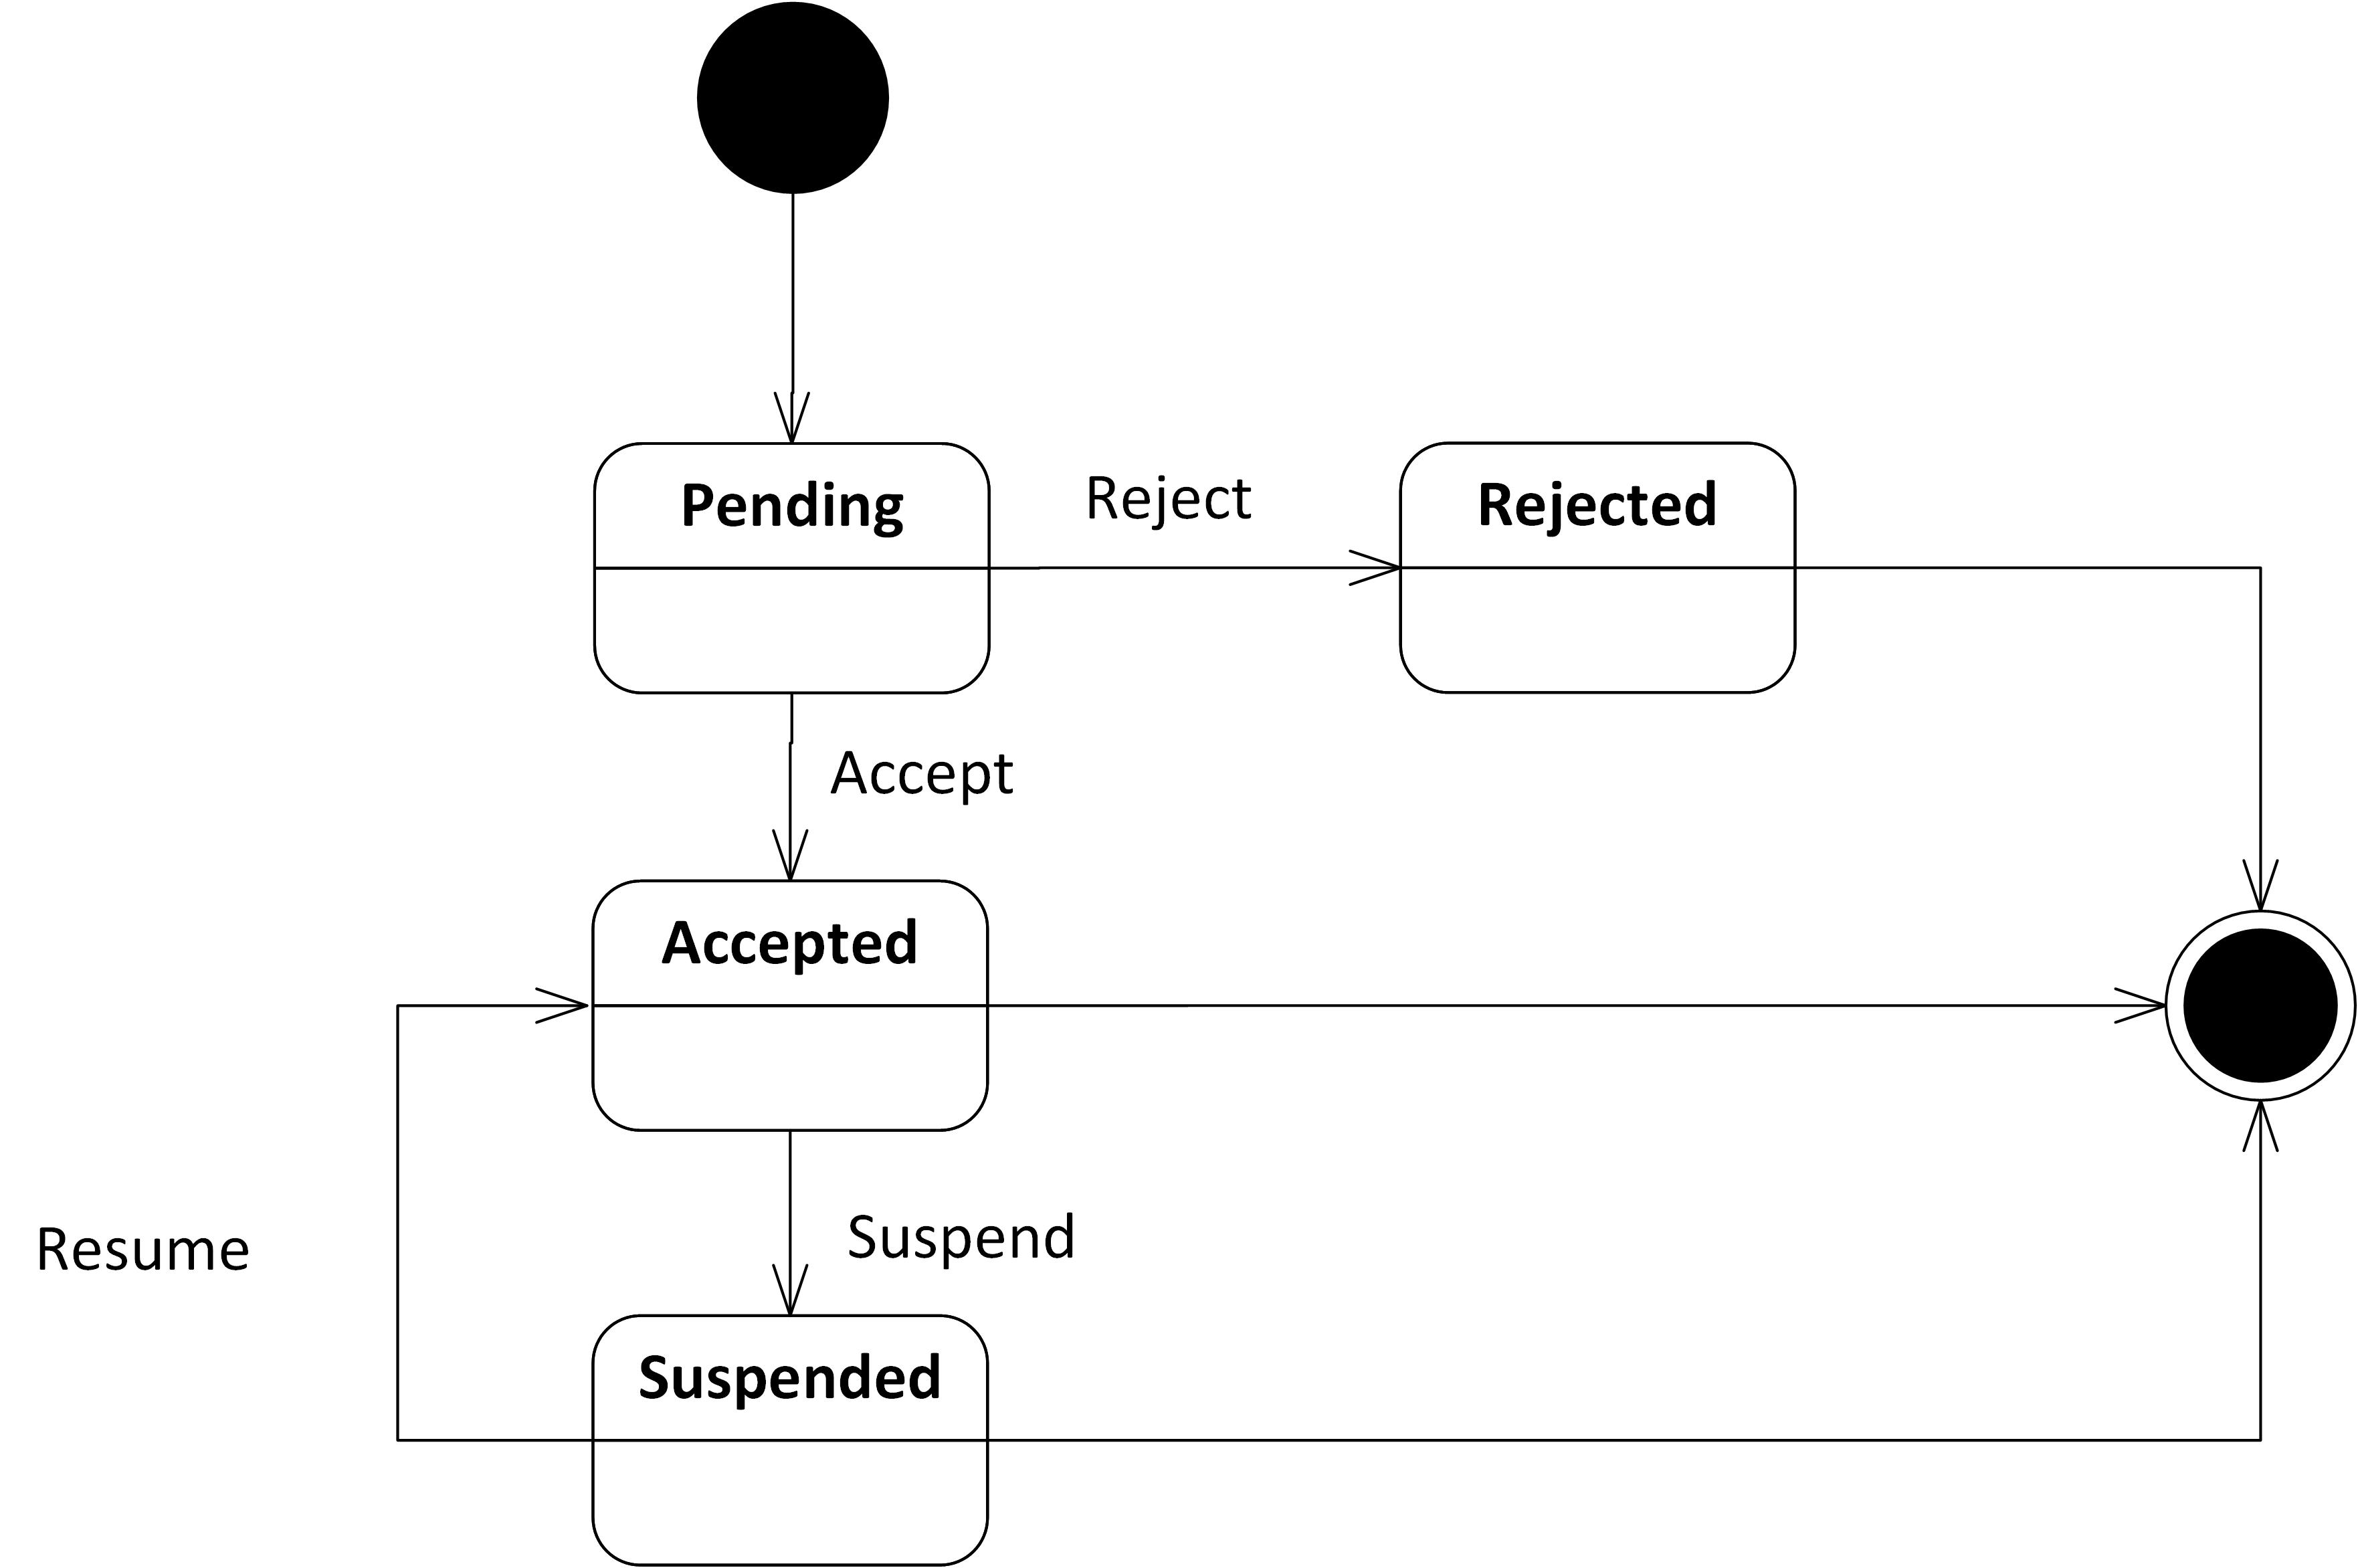
\includegraphics{figs/agreement-states.jpg}}} \par}
	\caption{State diagram for Agreement instance, inspired by WS-Agreement states \cite{ws-agreeement:2007} .}
	\label{fig:agreement-states}
\end{figure}


The actions that are applicable to \hl{Agreement} instances are presented in Table~\ref{tbl:agreement_actions}. The \hl{Action}s are defined by the \hl{Kind} instance \textit{http://schemas.ogf.org/occi/sla\#agreement}. Every \hl{Action} in the table is identified by a \hl{Category} instance using the \textit{http://schemas.ogf.org/occi/sla\#} categorization scheme. The “Action Term" below refers to the term of the \hl{Action}'s \hl{Category} identifier.


\mytablefloat{
	\label{tbl:agreement_actions}%
	\hl{Actions} applicable to instances of the \hl{Agreement} type.
}
{
	\begin{tabular}{lll}
	\toprule
	Action Term & Target state & Attributes \\
	\colrule
	accept & Accepted & -- \\
	reject & Rejected & -- \\
	suspend & Suspended & -- \\
	resume & Accepted & -- \\
	terminate & Terminated & -- \\
	\botrule
	\end{tabular}
}


These actions MUST be exposed by an instance of \hl{Agreement} type of an OCCI SLAs implementation. The implementation of the \hl{Agreement} type is REQUIRED if a cloud service provider adopts the OCCI SLAs specification.


\subsubsection{AgreementTemplate Mixin}
In order to allow the classification of agreements and the provisioning of Service Level Agreement templates, an OCCI \hl{Mixin} is introduced. The \hl{AgreementTemplate Mixin} is assigned the “scheme” \textit{http://schemas.ogf.org/occi/sla\#} and the term \hl{agreement\_tpl}. An \hl{AgreementTemplate} mixin MUST support these values. The use and instantiation of this \hl{Mixin} is OPTIONAL but RECOMMENDED for improved classification and management of the agreements.  There are no specific attributes defined for the \hl{AgreementTemplate Mixin}, thus every provider that implements the OCCI SLAs specification MAY introduce provider specific attributes using the Attributes Set inherited from the Category type.

As can be seen in the example diagram bellow, the \hl{AgreementTemplate} mixin can be used either for simple agreement tagging (e.g., gold, silver etc.) of a \hl{Collection} but also for introducing specific attributes and features for each tag.

\begin{figure}[!h]
	{\centering \resizebox*{0.9\columnwidth}{!}{{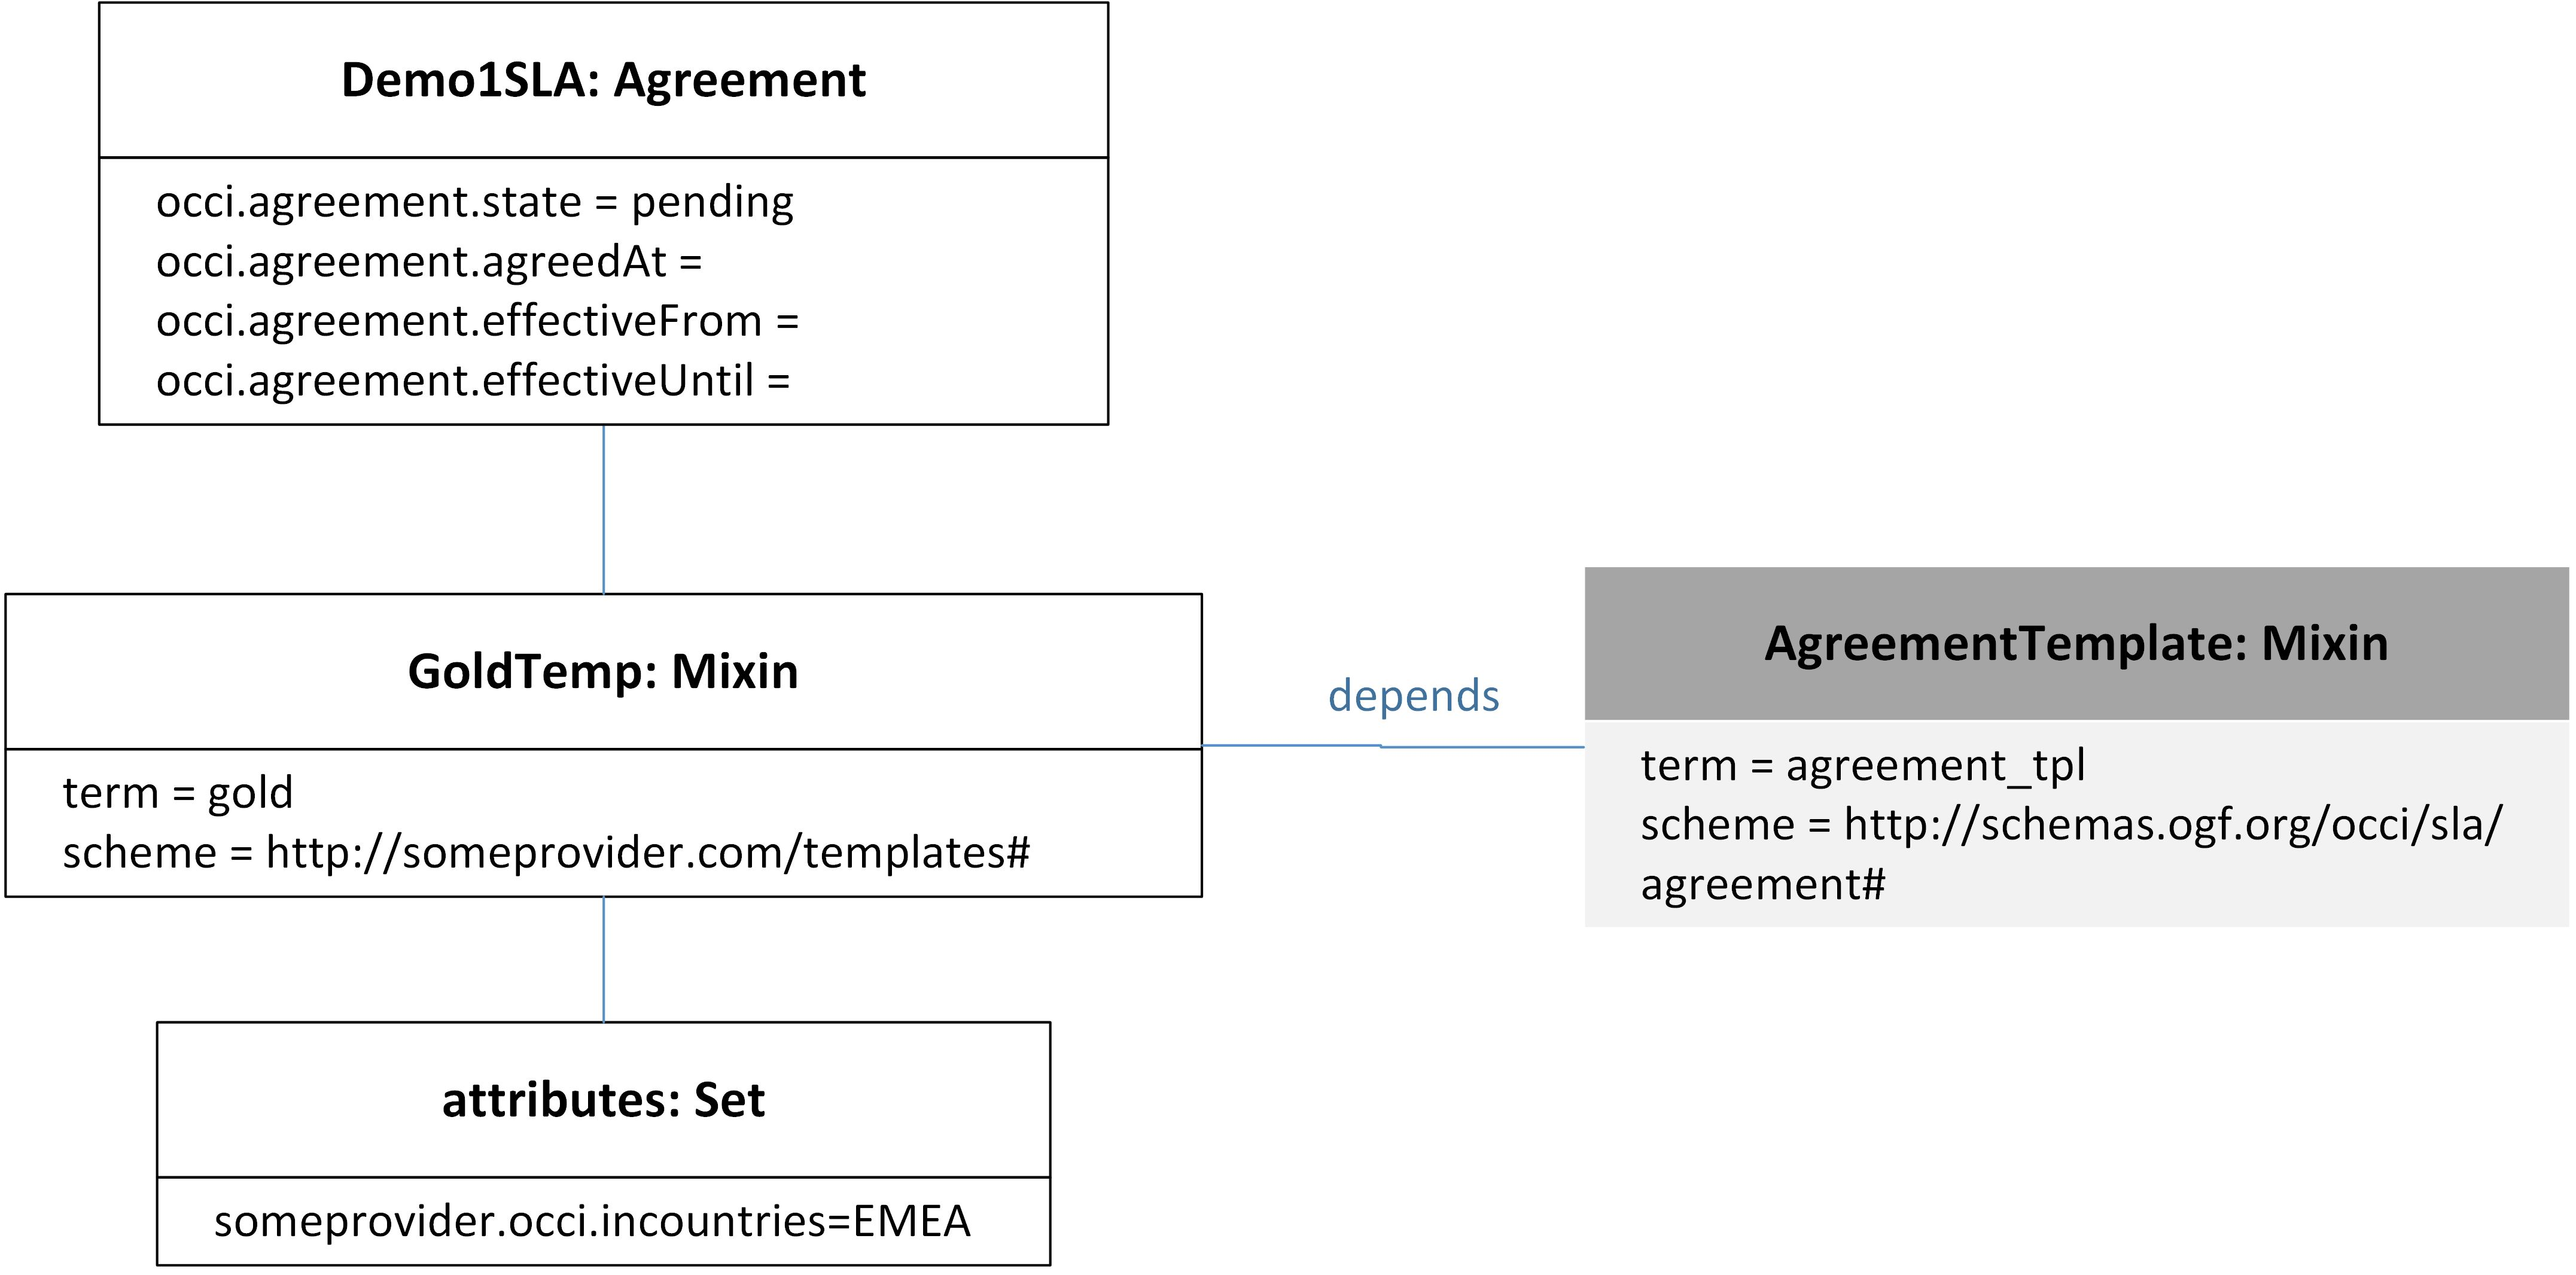
\includegraphics{figs/template-example.jpg}}} \par}
	\caption{Object diagram of an Agreement instance and its associated AgreementTemplate mixin.}
	\label{fig:template-example}
\end{figure}

\subsubsection{AgreementTerm Mixin}
A necessary part of an agreement offer, as well as the consequent agreement, is the section of the agreement term. To this end, the OCCI SLAs introduces the agreement terms through the \hl{Mixin} mechanism. The \hl{AgreementTerm Mixin} is assigned the “scheme” \textit{http://schemas.ogf.org/occi/sla\#} and the term \hl{agreement\_term}. An \hl{AgreementTerm} mixin MUST support these values. OCCI SLAs implementations SHOULD support this in order to provide a classification and definition mechanism for the various terms and conditions of the agreements. Therefore, the implementation of this functionality is OPTIONAL but RECOMMENDED.

While the Agreement Term Mixin as defined does not include any generic attribute, a provider specific term (e.g., availability, compute service term etc.) SHOULD be depended from the OCCI SLAs \hl{AgreementTerm Mixin} and introduce a set of attributes that characterize those terms. In Table~\ref{tbl:terms-attributes} a list of attributes is presented that a provider MAY use for the definition of the custom terms mixins. Following the rationale presented in the WS-Agreement specification \cite{ws-agreeement:2007} , OCCI SLAs defines two types of agreement terms: service terms and service level objectives (SLOs). The first includes information related with the service description and definition. The second refers to the guarantee terms that specify the service level which the two parties are agreeing to. A cloud service provider MAY introduce more domain specific attributes to the \hl{AgreementTerm} mixin instances that he constructs, through the attributes set inherited from the \hl{Category} type. \hl{Mixin} relationships MAY be used in order to enforce classification of capabilities but also to allow resource specific instantiation of \hl{AgreementTerm}. For example, an availability \hl{Mixin} could be defined, which is depended on the \hl{AgreementTerm Mixin} type. The provider, then, MAY choose to instantiate different availability mixins for compute or storage resources (or any other offered resource) based on his own definition of availability for those resources.



\mytablefloat{
	\label{tbl:terms-attributes}
	Suggested \hl{Attributes} for a provider-defined AgreementTerm Mixin.
}
{
	\begin{tabular}{lp{2.5cm}p{1cm}lp{6cm}}
	\toprule
	Attribute&Type&Multi\-plicity&Mutability&Description\\
	\colrule
	\{term\_name\}.term.type & Enum \{SERVICE-TERM,SLO-TERM, n/a\} & 1 & Immutable & The type of the term that is being defined.\\
	\{term\_name\}.term.state & Enum \{Undefined, Fulfilled, Violated\} & 1 & Immutable & The state of fulfillment of the specific term. \\
	\{term\_name\}.term.desc & String & 0\ldots1 & Immutable & The description of the agreement term defined with this mixin. \\
	\{term\_name\}.term.remedy & String & 0\ldots1 & Immutable & The remedy value (e.g., price penalty) or action e.g., command) when an SLO term is being violated. \\
	\botrule
	\end{tabular}
}



The \hl{AgreementTerm} state can be either \textit{undefined}, \textit{fulfilled} or \textit{violated} (Figure~\ref{fig:terms-states}). The undefined state is the initial state of the term until an assessment is made. During runtime and while the service and SLA is being monitored the state MUST be fulfilled or violated. When multiple terms exist (e.g., provider specific terms) then if at least one term in an agreement has state violated, then the agreement is considered violated (\textit{\{term\_name\}.term.state=violated}).

\begin{figure}[!h]
	{\centering \resizebox*{0.6\columnwidth}{!}{{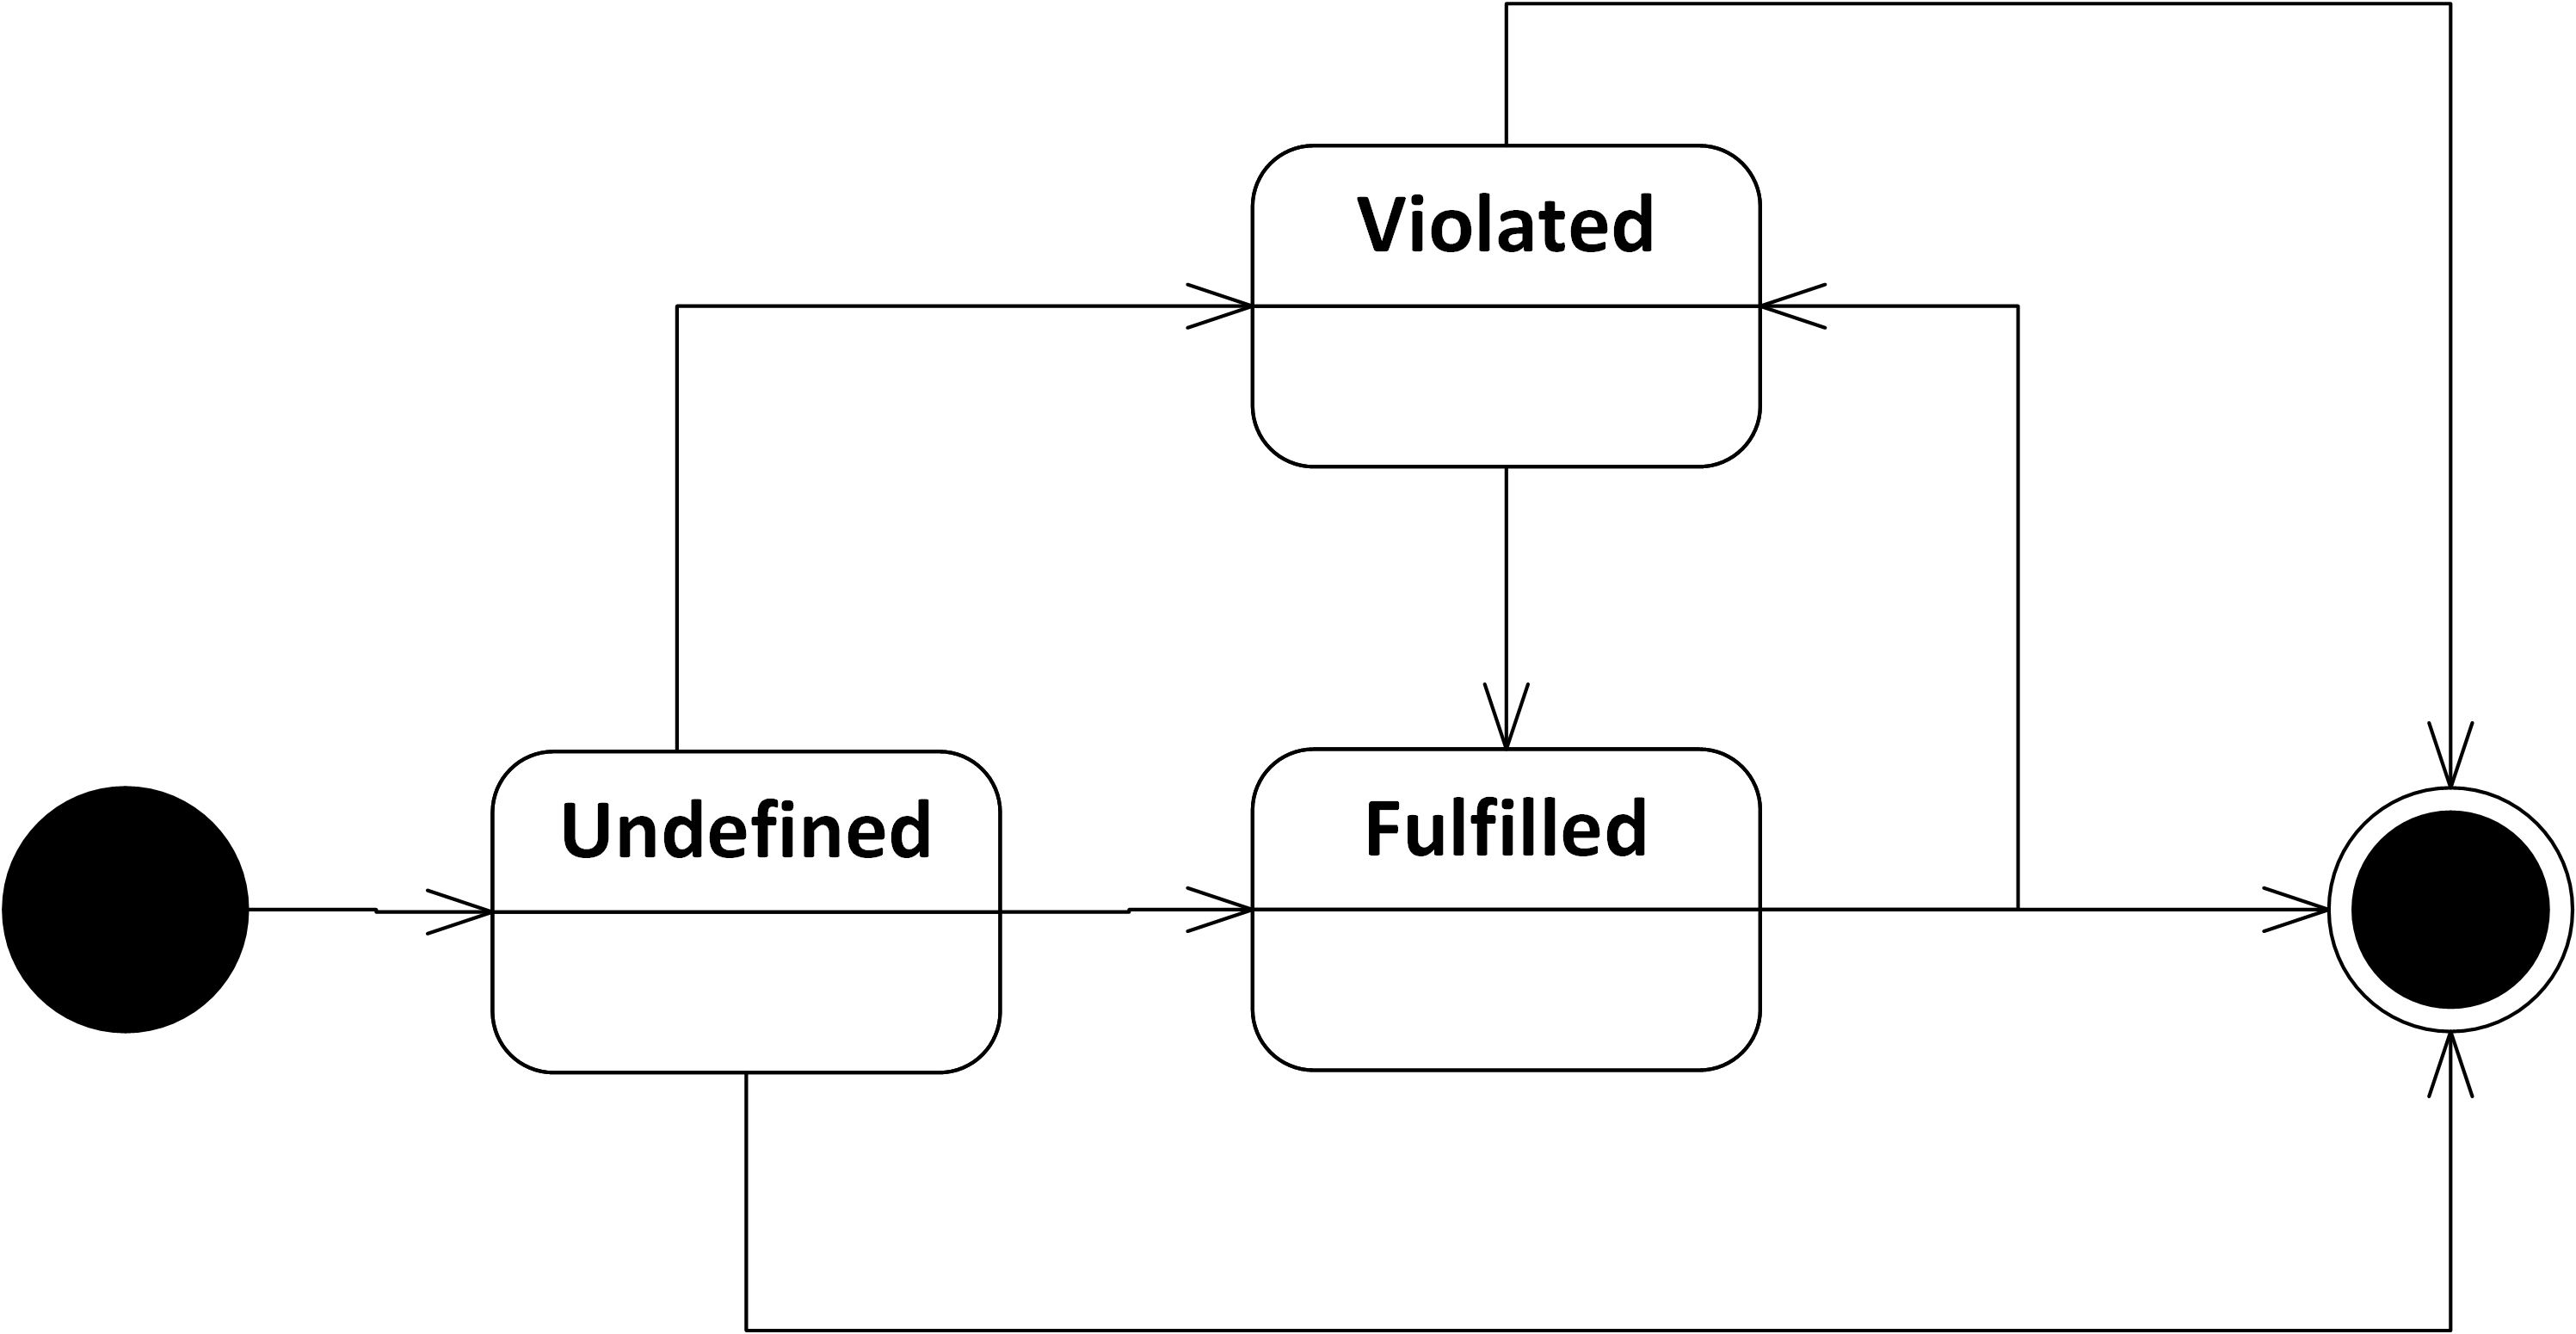
\includegraphics{figs/terms-states.jpg}}} \par}
	\caption{AgreementTerm state diagram.}
	\label{fig:terms-states}
\end{figure}

In Figure~\ref{fig:terms-example} an example of using the \hl{AgreementTerm Mixin} is shown. In the specific implementation an agreement offer (state: pending) is defined which describes a SLA for a compute service (memory: 16GB, cores: 4). The \textit{Availability} Service Level Objective (SLO) is introduced through provider specific attributes in the respective mixin.

\begin{figure}[!h]
	{\centering \resizebox*{0.95\columnwidth}{!}{{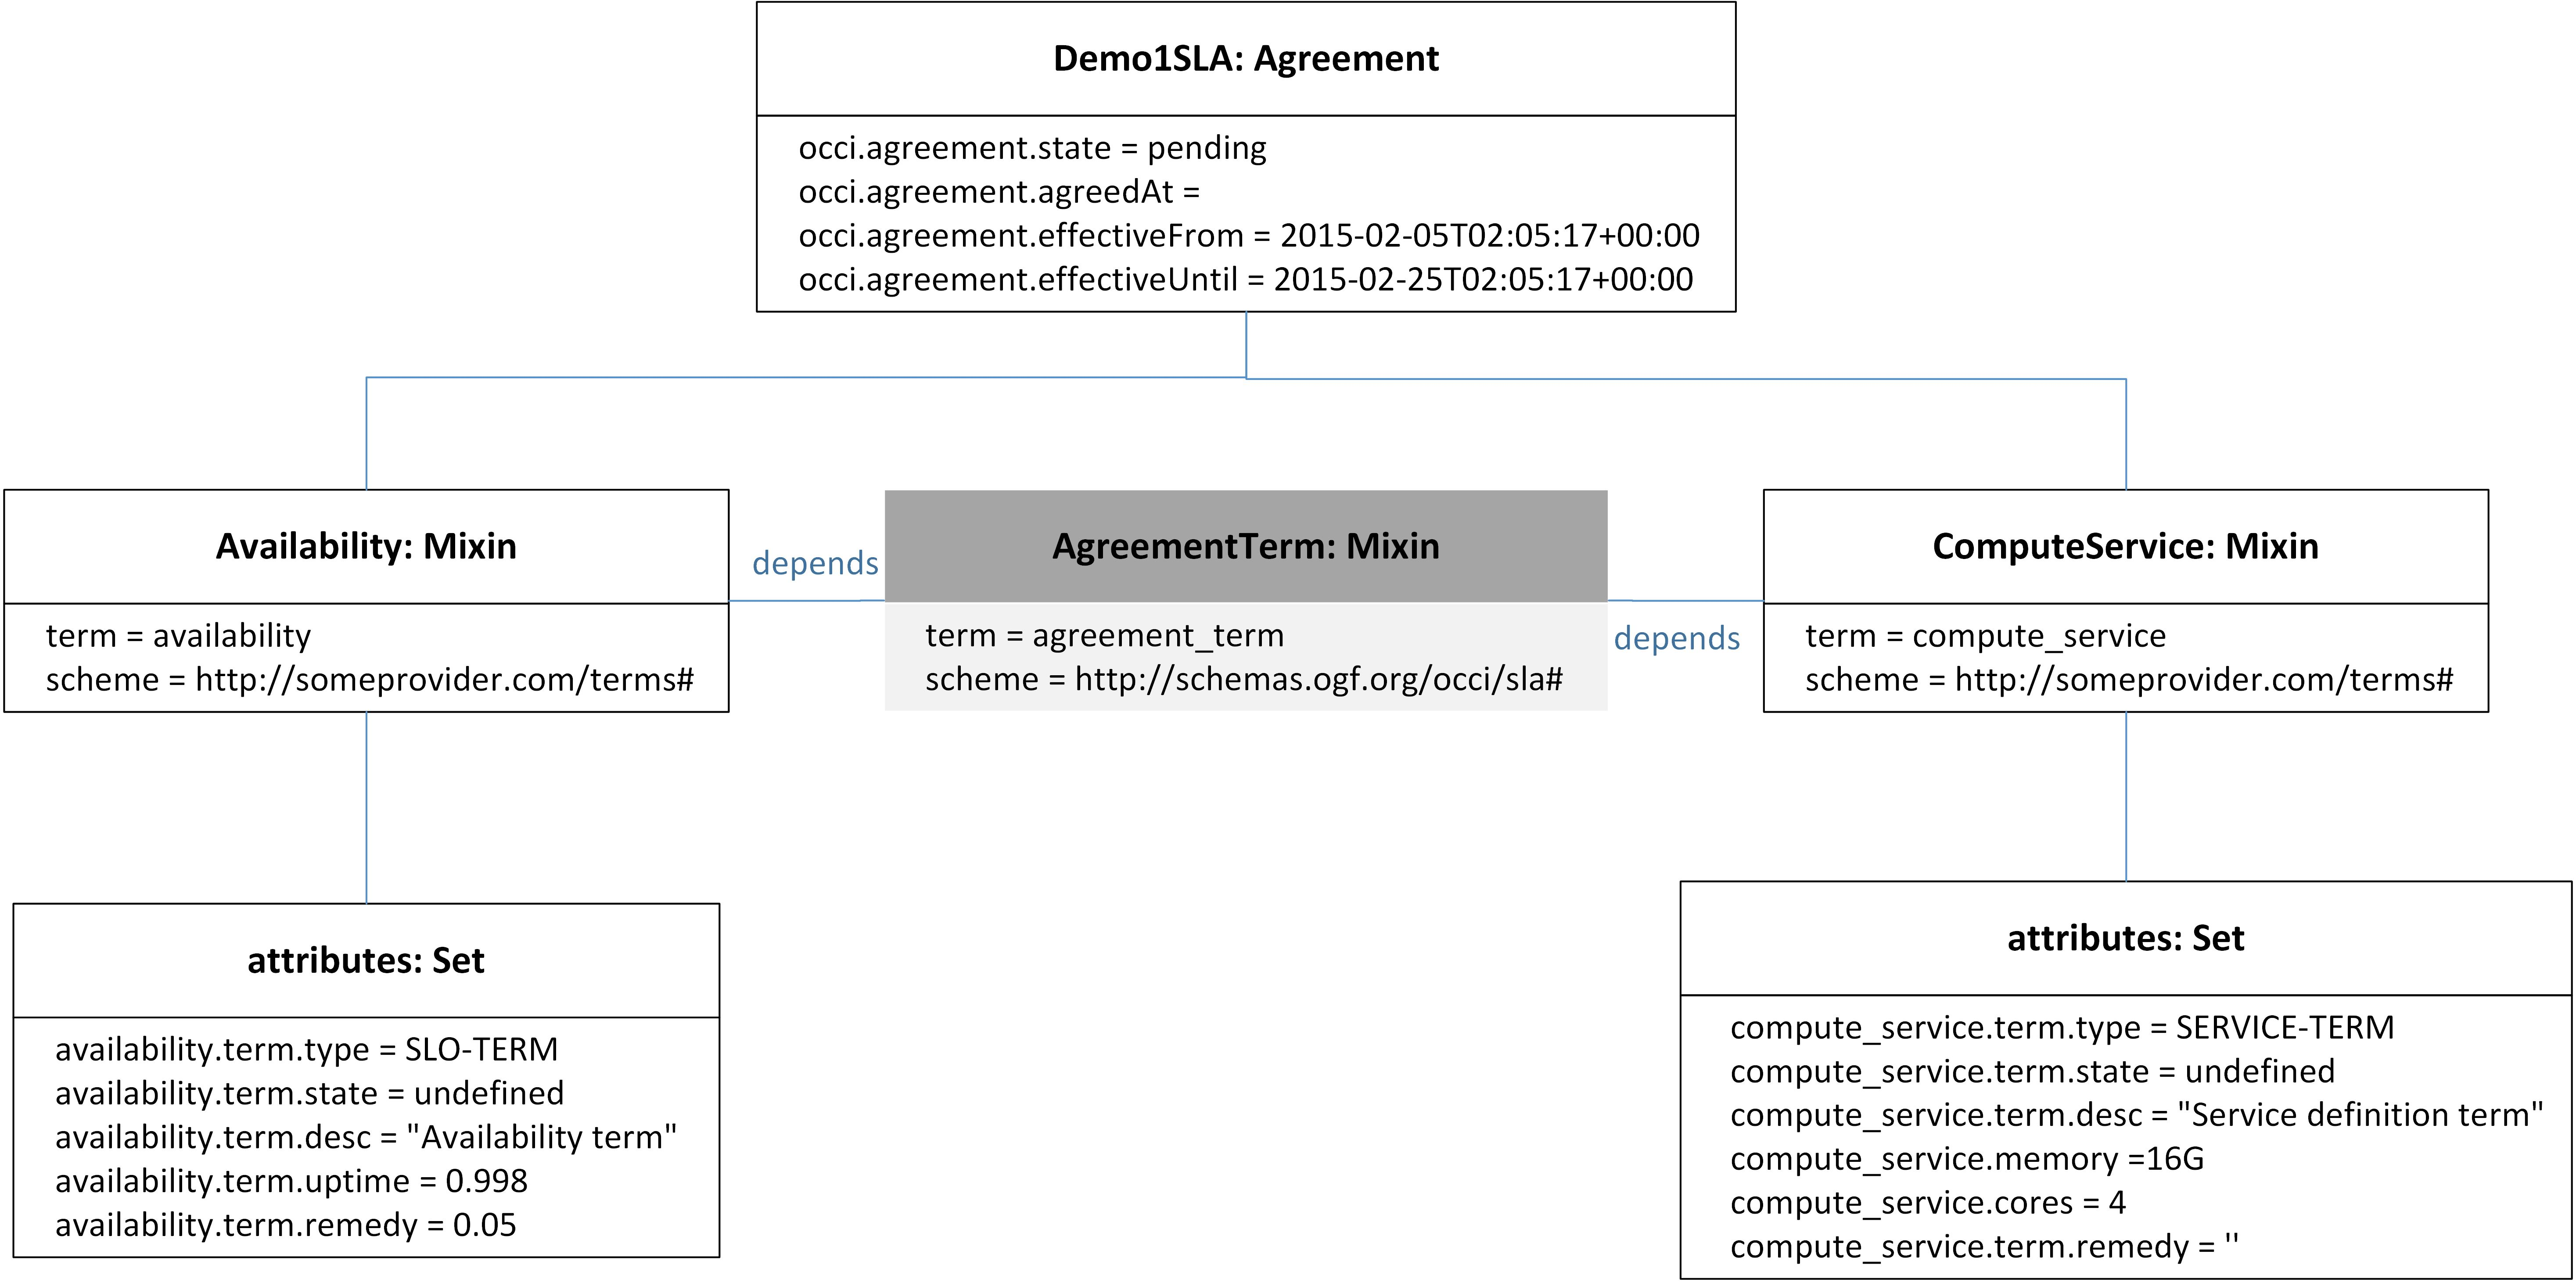
\includegraphics{figs/terms-example.jpg}}} \par}
	\caption{Object diagram of an Agreement instance populated with AgreementTerm mixin.}
	\label{fig:terms-example}
\end{figure}


\subsection{AgreementLink}
In order to associate signed Service Level Agreements with existing OCCI resource instances, the \hl{AgreementLink} is introduced. This is a sub-type of the OCCI Core Model Link base type. Thus, the instantiation of an \hl{AgreementLink} resource allows the linkage of resources of the previous defined \hl{Agreement} sub-type with any OCCI Core Model Resource sub-type (e.g., Infrastructure sub-types). The implementation of the \hl{AgreementLink} type is REQUIRED if a cloud service provider adopts the OCCI SLAs specification.

The \hl{AgreementLink} type is assigned the \hl{Kind} instance \textit{http://schemas.ogf.org/occi/sla\#agreement\_link}. An \hl{AgreementLink} instance MUST use and expose this Kind. The \hl{Kind} instance assigned to the \hl{AgreementLink} type MUST be related to the \textit{http://schemas.ogf.org/occi/core\#link} \hl{Kind}.

Because of the multiple possibilities in terms of design and implementation of an OCCI compatible system, domain specific AgreementLink sub-types MAY be defined by cloud service providers. Thus, additional, provider specific attributes in such agreement link sub-types MAY be defined in by its Kinds instances.


\subsection{OCCI Service Level Agreement example}

In this section, an example instantiation of an Agreement type along with provider defined mixins is presented. It is to be noted that the implementation of an OCCI SLA framework is a responsibility of the cloud service provider. Thus, the instantiation of the proposed types and mixins are subject to the requirements and objectives of the provider. The presented instantiation of an OCCI SLA is only an example. Different approaches, mixins and attributes definitions could be followed.

The creation and provisioning of SLAs includes several phases.  The process of reaching such agreement could be described by the following steps :
\begin{itemize}
\item Negotiation phase -- The cloud service consumer retrieves the SLA templates, completes the REQUIRED values and submits an offer to the cloud service provider. (agreement-state: pending)
\item Agreement phase -- The cloud service provider can decide whether to accept the filled out template (the offer) or not. It is also possible to provide a counter-offer to the customer. (agreement-state: accepted, rejected, pending)
\item Execution phase -- When the agreement has been accepted the Agreement is in place and the (newly) created resource can be linked and associated with the reached agreement. (agreement-state: accepted)
\end{itemize}
The object diagram in Figure~\ref{fig:occi-slas-example} represents an Agreement in the execution phase. In the presented example the Demo1SLA agreement is being populated with the SilverTemp mixin which is related to the AgreementTemplate Mixin type. This is used to tag and classify the agreement as well as to define some generic constraints such as the region in which the resources (under that SLA template) SHOULD be allocated. In addition to the template mixin several AgreementTerm mixins are defined either to define and describe the service offered or to introduce Service Level Objectives (SLOs) for the agreement.

To this end, through the \textit{ComputeServiceTerm} mixin, the cloud service provider introduces a set of service terms which characterize the service being offered with this SLA. In this case it is a compute resource with technical specifications defined through provider-specific attributes (e.g., \textit{compute\_service.cores}, \textit{compute\_service.cpu} etc.). The \textit{Availability}, \textit{ServicePerformance} and \textit{ServiceCapacity} are all Service Level Objective terms that set certain thresholds to metrics which determine the Quality of Service (QoS) of the respective offering. Every SLO term also defines the remedy value which is the compensation to the costumer in the event that the cloud service provider fails to meet the specified SLO. The value is usually a percentage of the agreed rate for the offered cloud service. The attributes defined in the mixins can be either mutable or immutable to the costumer depending on how the negotiation phase is being realized by the cloud service provider. What is more, every term has a current state value. Depending on the current assessment the terms are fulfilled or violated. Each violation will trigger the respective remedy value.

\begin{figure}[!h]
	{\centering \resizebox*{0.9\columnwidth}{!}{\rotatebox{270}{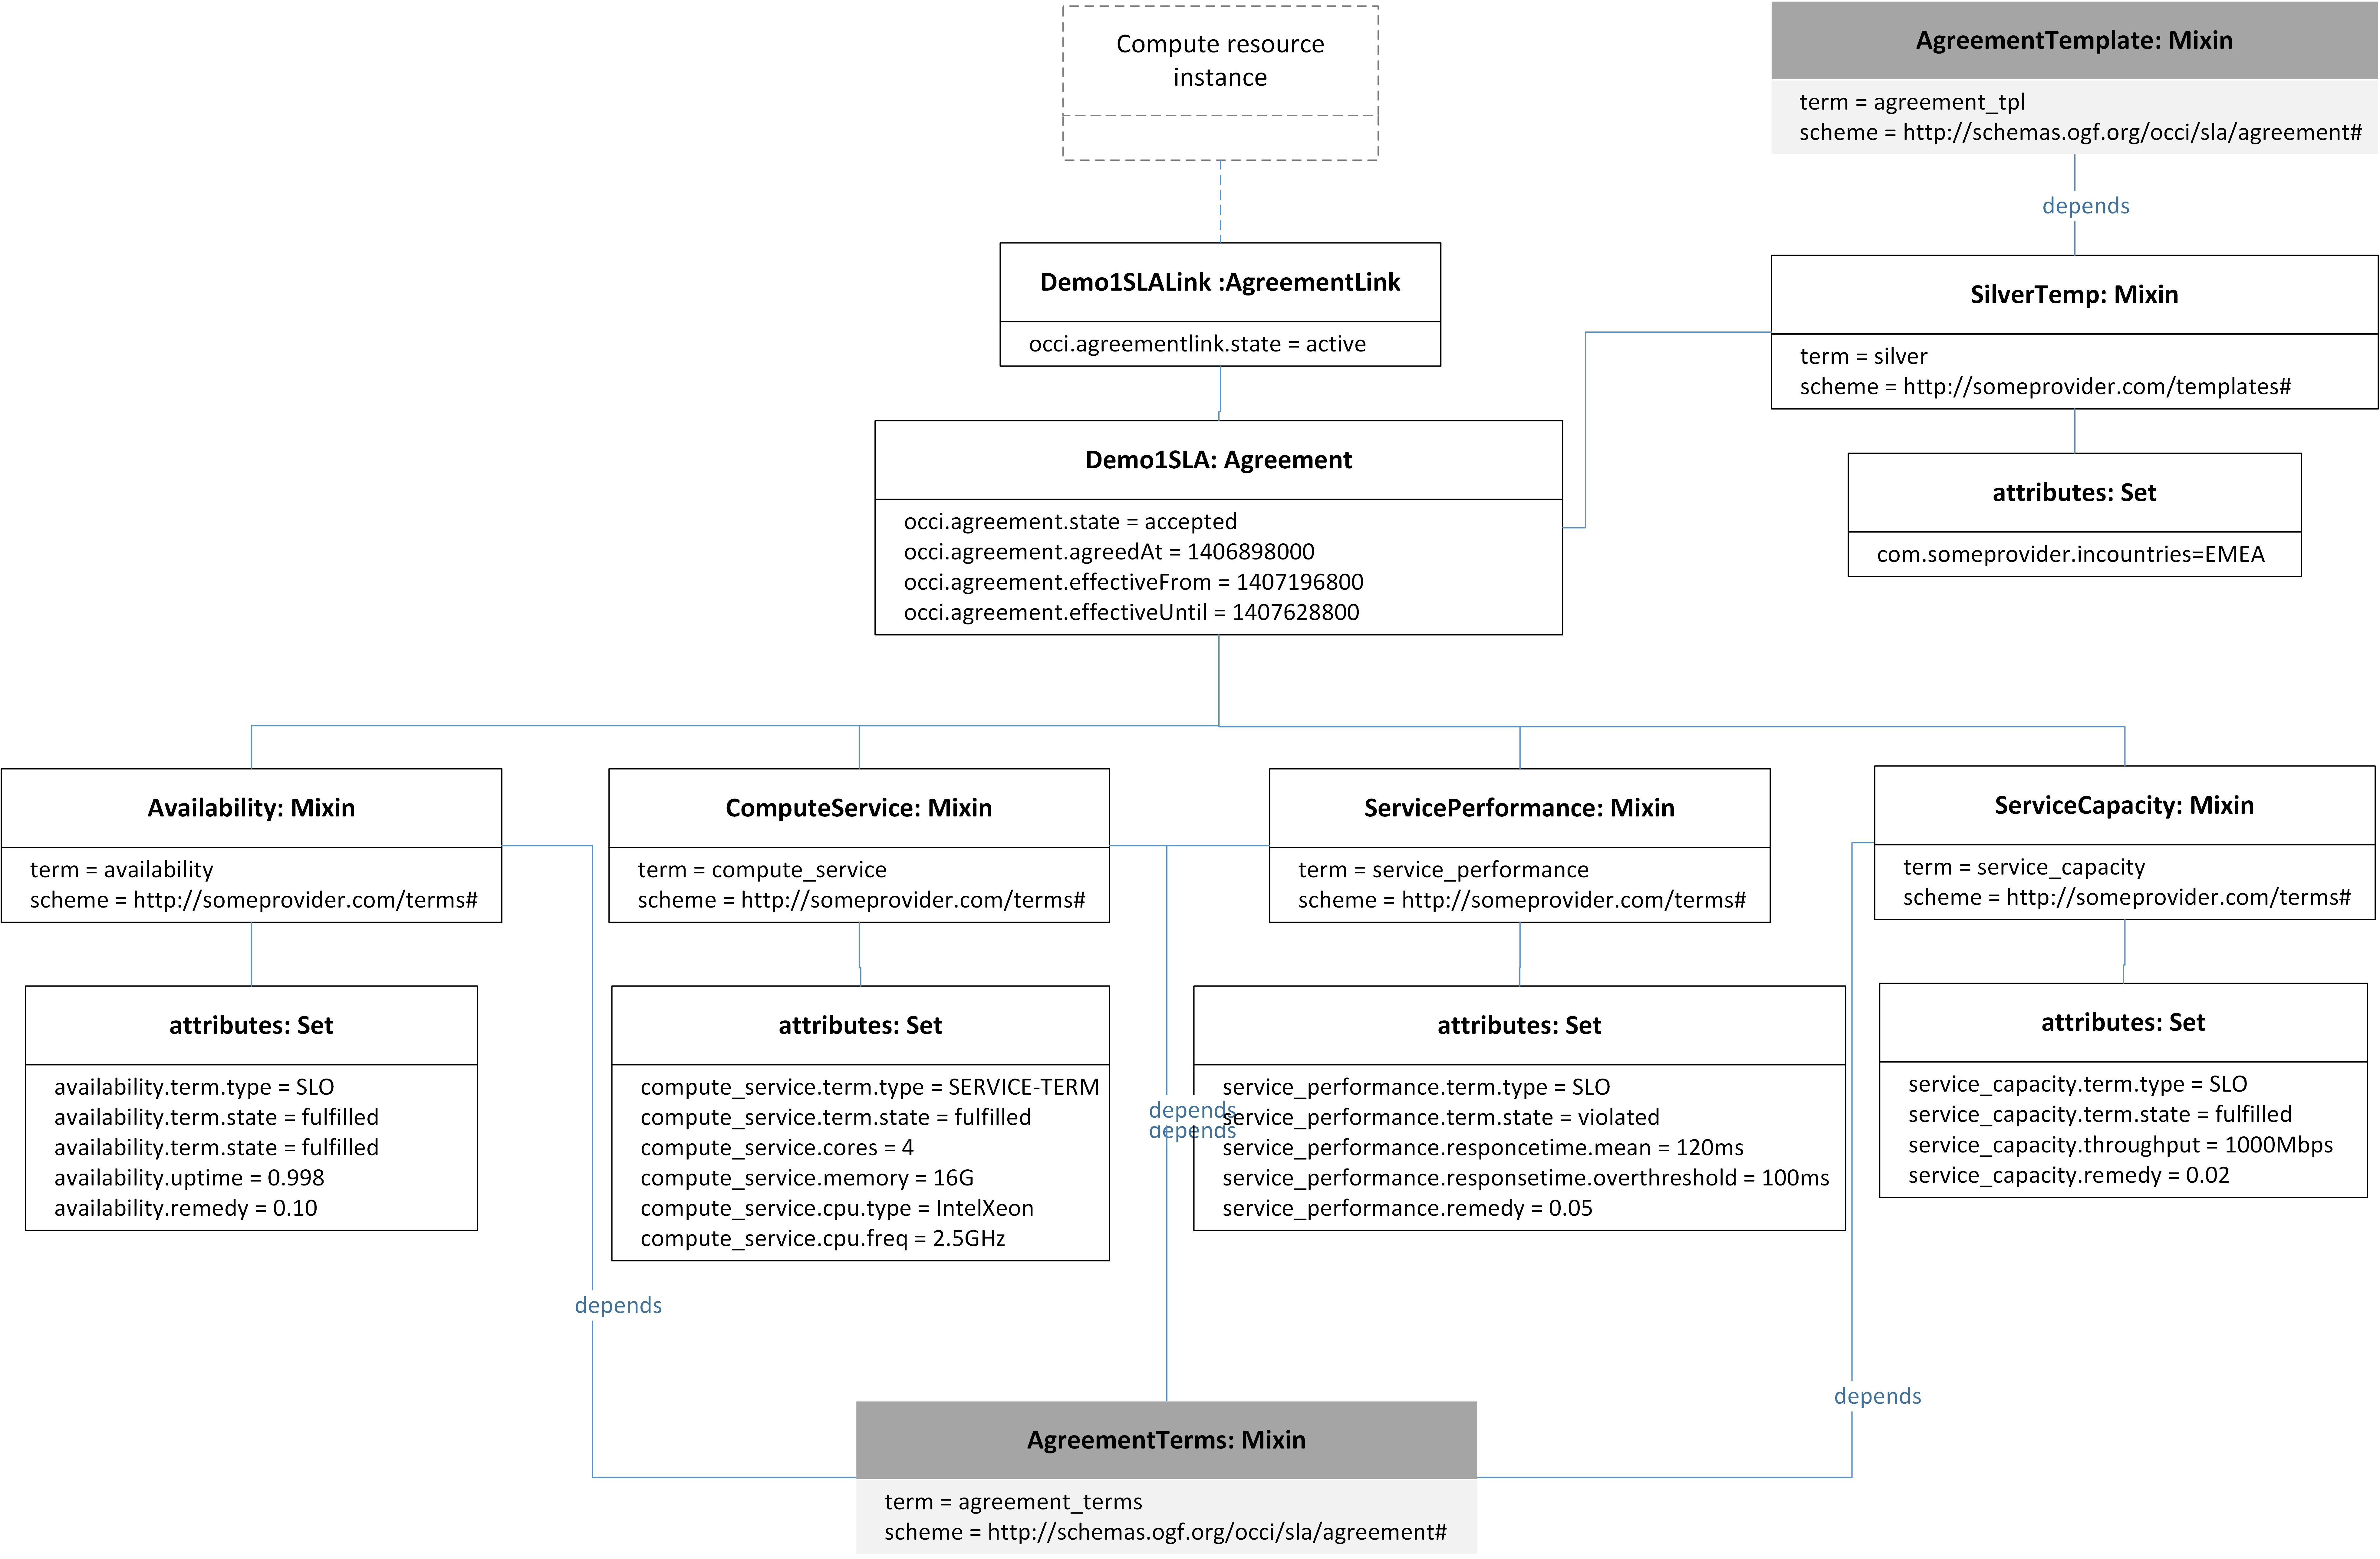
\includegraphics{figs/occi-slas-example.jpg}}} \par}
	\caption{OCCI SLA instantiation example.}
	\label{fig:occi-slas-example}
\end{figure}



% end sla content

\section{Security Considerations}
The OCCI Infrastructure specification is an extension to the OCCI Core
and Model specification \cite{occi:core}; thus the same security
considerations as for the OCCI Core and Model specification apply
here.

\section{Glossary}
\label{sec:glossary}

\section{Glossary}
\label{s:glossary}

\begin{description}
\item[metric] a metric is a mathematical representation of a well defined aspect of a physical entity
\item[measurement] a measurement is the process of extracting a metric from a physical entity, and by extension also the result of such process. The measurement seldom corresponds exactly to the value of the metric.
\item[SLA] {\em ``An agreement defines a dynamically-established and dynamically
managed relationship between parties. The object of this
relationship is the delivery of a service by one of the parties within
the context of the agreement.''} from {\em SLA@SOI Glossary}
\item[Restful model] {\em ``REST is a coordinated set of architectural constraints that attempts to minimize latency and network communication, while at the same time maximizing
the independence and scalability of component implementations.''} \cite{fie02a}
\item[OCCI] {``\em The Open Cloud Computing Interface (OCCI) is a RESTful Protocol and API for all kinds of management tasks. OCCI was originally initiated to create a remote management API for IaaS model-based services, allowing for the development of interoperable tools for common tasks including deployment, autonomic scaling and monitoring''} \cite{occi:core}
\item[OCCI {\em Kind}] {\em''The Kind type represents the type identification mechanism for all Entity types present in the model''} \cite{occi:core}
\item[OCCI {\em \ln}] {\em''An instance of the Link type defines a base association between two Resource instances.''} \cite{occi:core}
\item[OCCI \mi] {\em''The Mixin type represent an extension mechanism, which allows new resource
capabilities to be added to resource instances both at creation-time and/or run-time.''} \cite{occi:core}
\item[OCCI \rs] {\em''A Resource is suitable to represent real world resources, e.g. virtual machines, networks, services, etc. through specialisation.''} \cite{occi:core}
\item[\sens] The \sens\ is a \rs\ that collects metrics from its input side, and delivers aggregated metrics from its output
\item[\coll] The \coll\ is a link that conveys metrics: it defines both the transport protocol and the conveyed metrics.
\end{description}


\section{Contributors}
%
We would like to thank the following people who contributed to this
document:

\begin{tabular}{l|p{2in}|p{2in}}
Name & Affiliation & Contact \\
\hline
Michael Behrens & R2AD & behrens.cloud at r2ad.com \\
Mark Carlson & Toshiba & mark at carlson.net \\
Augusto Ciuffoletti & University of Pisa & augusto.ciuffoletti at gmail.com\\
Andy Edmonds & ICCLab, ZHAW & edmo at zhaw.ch \\
Sam Johnston & Google & samj at samj.net \\
Gary Mazzaferro & Independent &  garymazzaferro at gmail.com \\
Thijs Metsch & Intel & thijs.metsch at intel.com \\
Ralf Nyrén & Independent & ralf at nyren.net \\
Alexander Papaspyrou & Adesso & alexander at papaspyrou.name \\
Boris Parák & CESNET & parak at cesnet.cz \\
Alexis Richardson & Weaveworks & alexis.richardson at gmail.com \\
Shlomo Swidler & Orchestratus & shlomo.swidler at orchestratus.com \\
Florian Feldhaus & Independent & florian.feldhaus at gmail.com \\
Zden\v{e}k \v{S}ustr & CESNET & zdenek.sustr at cesnet.cz \\
\end{tabular}

Next to these individual contributions we value the contributions from
the OCCI working group.


%--- occi slas contributors ---
We would like to thank the following people who contributed to this document:

\begin{tabular}{l|p{2in}|p{2in}}
Name & Affiliation & Contact \\
\hline
Gregory Katsaros & Intel & gregory.katsaros at intel.com \\
Thijs Metsch & Intel & thijs.metsch at intel.com \\
John Kennedy & Intel & john.m.kennedy at intel.com \\
Alexander Stanik & TU Berlin & alexander.stanik at tu-berlin.de \\
Wolfgang Ziegler & SCAI Fraunhofer & wolfgang.ziegler at scai.fraunhofer.de \\
\end{tabular}

Next to these individual contributions we value the contributions from the OCCI working group.

\section{Intellectual Property Statement}
The OGF takes no position regarding the validity or scope of any
intellectual property or other rights that might be claimed to pertain
to the implementation or use of the technology described in this
document or the extent to which any license under such rights might or
might not be available; neither does it represent that it has made any
effort to identify any such rights. Copies of claims of rights made
available for publication and any assurances of licenses to be made
available, or the result of an attempt made to obtain a general
license or permission for the use of such proprietary rights by
implementers or users of this specification can be obtained from the
OGF Secretariat.

The OGF invites any interested party to bring to its attention any
copyrights, patents or patent applications, or other proprietary
rights which may cover technology that may be required to practice
this recommendation. Please address the information to the OGF
Executive Director.


\section{Disclaimer}
This document and the information contained herein is provided on an
``As Is'' basis and the OGF disclaims all warranties, express or
implied, including but not limited to any warranty that the use of the
information herein will not infringe any rights or any implied
warranties of merchantability or fitness for a particular purpose.


\section{Full Copyright Notice}
Copyright \copyright ~Open Grid Forum (2009-2011). All Rights Reserved.

This document and translations of it may be copied and furnished to
others, and derivative works that comment on or otherwise explain it
or assist in its implementation may be prepared, copied, published and
distributed, in whole or in part, without restriction of any kind,
provided that the above copyright notice and this paragraph are
included on all such copies and derivative works. However, this
document itself may not be modified in any way, such as by removing
the copyright notice or references to the OGF or other organizations,
except as needed for the purpose of developing Grid Recommendations in
which case the procedures for copyrights defined in the OGF Document
process must be followed, or as required to translate it into
languages other than English.

The limited permissions granted above are perpetual and will not be
revoked by the OGF or its successors or assignees.


\bibliographystyle{IEEEtran}
\bibliography{references}

\appendix


\end{document}
